\documentclass[UTF8,a4paper,zihao=5,fontset=fandol]{ctexart}
\usepackage[top=20mm,bottom=21mm,left=22mm,right=22mm]{geometry}
\usepackage{amsmath,amssymb,booktabs,tabularx,array,multirow,graphicx,xcolor,caption,cite,placeins,float,hyperref}
\setmainfont{TeX Gyre Termes}
\setsansfont{TeX Gyre Heros}
\hypersetup{colorlinks=false,pdfborder={0 0 0.6},linkbordercolor={1 0 0},citebordercolor={0 1 0},urlbordercolor={0 1 1},pdfhighlight=/I,bookmarksnumbered=true,pdftitle={基于域内预训练与标记条件学习的DAPI虚拟染色},pdfauthor={通信速通生物}}
\ctexset{section={format=\large\bfseries,beforeskip=11pt,afterskip=6pt},subsection={format=\normalsize\bfseries,beforeskip=8pt,afterskip=4pt},subsubsection={format=\normalsize\bfseries,beforeskip=6pt,afterskip=3pt}}
\captionsetup{font=small,labelfont=bf,labelsep=period,skip=5pt}
\setlength{\parskip}{2pt}\setlength{\parindent}{2em}
\setlength{\emergencystretch}{2em}
\setlength{\textfloatsep}{11pt plus 2pt minus 2pt}
\setlength{\dbltextfloatsep}{12pt plus 2pt minus 2pt}
\setlength{\abovedisplayskip}{6pt}\setlength{\belowdisplayskip}{5pt}
\postdisplaypenalty=10000
\raggedbottom
\renewcommand{\arraystretch}{1.13}\linespread{1.06}
\newcolumntype{Y}{>{\raggedright\arraybackslash}X}
\newcommand{\op}[1]{\operatorname{#1}}
\newcommand{\sym}[1]{\par\nobreak\noindent\begin{minipage}{\linewidth}#1\end{minipage}\par}
\newcommand{\code}[1]{\texttt{\detokenize{#1}}}
\pagestyle{plain}
\begin{document}
\begin{center}
{\LARGE\bfseries 基于域内预训练与标记条件学习的 DAPI 虚拟染色}\par
\vspace{9pt}
{\large 通信速通生物}\par\vspace{5pt}
通信速通生物\quad AIC-2026-51865112\par
\vspace{9pt}
\end{center}


\begin{abstract}
针对结肠、肝脏和胃组织的 DAPI 虚拟染色任务，本文构建以目标标记为条件的共享预测网络。网络以 ConvNeXt V2 为主干，通过跳跃连接与像素重排恢复分辨率，并以目标标记嵌入调制多尺度编码特征。完整流程包括按组织区域划分数据、DAPI 域内掩码重建预训练、ROI 留出教师监督训练与目标生成，以及全量学生监督训练。学生先学习真实标签，再结合教师预测与几何一致性约束优化染色映射；推理使用固定学生模型，从完整单张 DAPI 生成指定标记图像。结肠与胃选择 CD68，肝脏选择 CD45RO。在固定 ROI 验证划分上，引入蒸馏后的综合分数为 76.2247，加入并加强几何一致性约束后达到 76.2807。最终全量学生的平台加权分数为 74.0677，结肠、肝脏和胃的分数分别为 73.1963、78.7011 和 72.8684。
\end{abstract}

\section{任务背景与方法概览}\label{sec:overview}
本节介绍 DAPI 虚拟染色任务，并概述网络设计及训练、推理流程。
DAPI 图像提供细胞核及其空间分布信息，虚拟染色模型通过配对训练学习这些形态信息与目标免疫标记之间的关系。本方案面向结肠、肝脏和胃数据，将三个器官的训练样本用于同一个条件模型。每次预测以一张 DAPI 和一个目标标记编号为输入，生成一张同尺寸的目标图像。

网络采用 U 型多尺度特征融合思路\cite{unet}，参考 Cytoland 中面向显微图像翻译的 UNeXt2 设计\cite{cytoland}，以 ConvNeXt V2 块构建编码器和解码器\cite{convnext}。域内预训练采用全卷积掩码自编码（fully convolutional masked autoencoder，FCMAE）目标。上采样采用子像素重排\cite{espcn}，条件注入采用特征逐通道线性调制（feature-wise linear modulation，FiLM）\cite{film}。本文在上述结构基础上，以目标标记嵌入调制四级编码特征，并通过图像回归蒸馏和训练阶段的几何一致性约束学习共享染色映射。

这些设计分别对应表征、任务区分和输出稳定性三个方面：域内预训练利用 DAPI 重建信号学习显微形态表征，标记条件指定期望的染色目标，教师预测提供辅助回归目标。几何一致性进一步约束旋转、翻转前后的预测关系，使网络在训练中学习与图像方向变换相协调的染色映射。图\ref{fig:workflow}概括了完整流程。

\begin{figure}[htbp]\centering
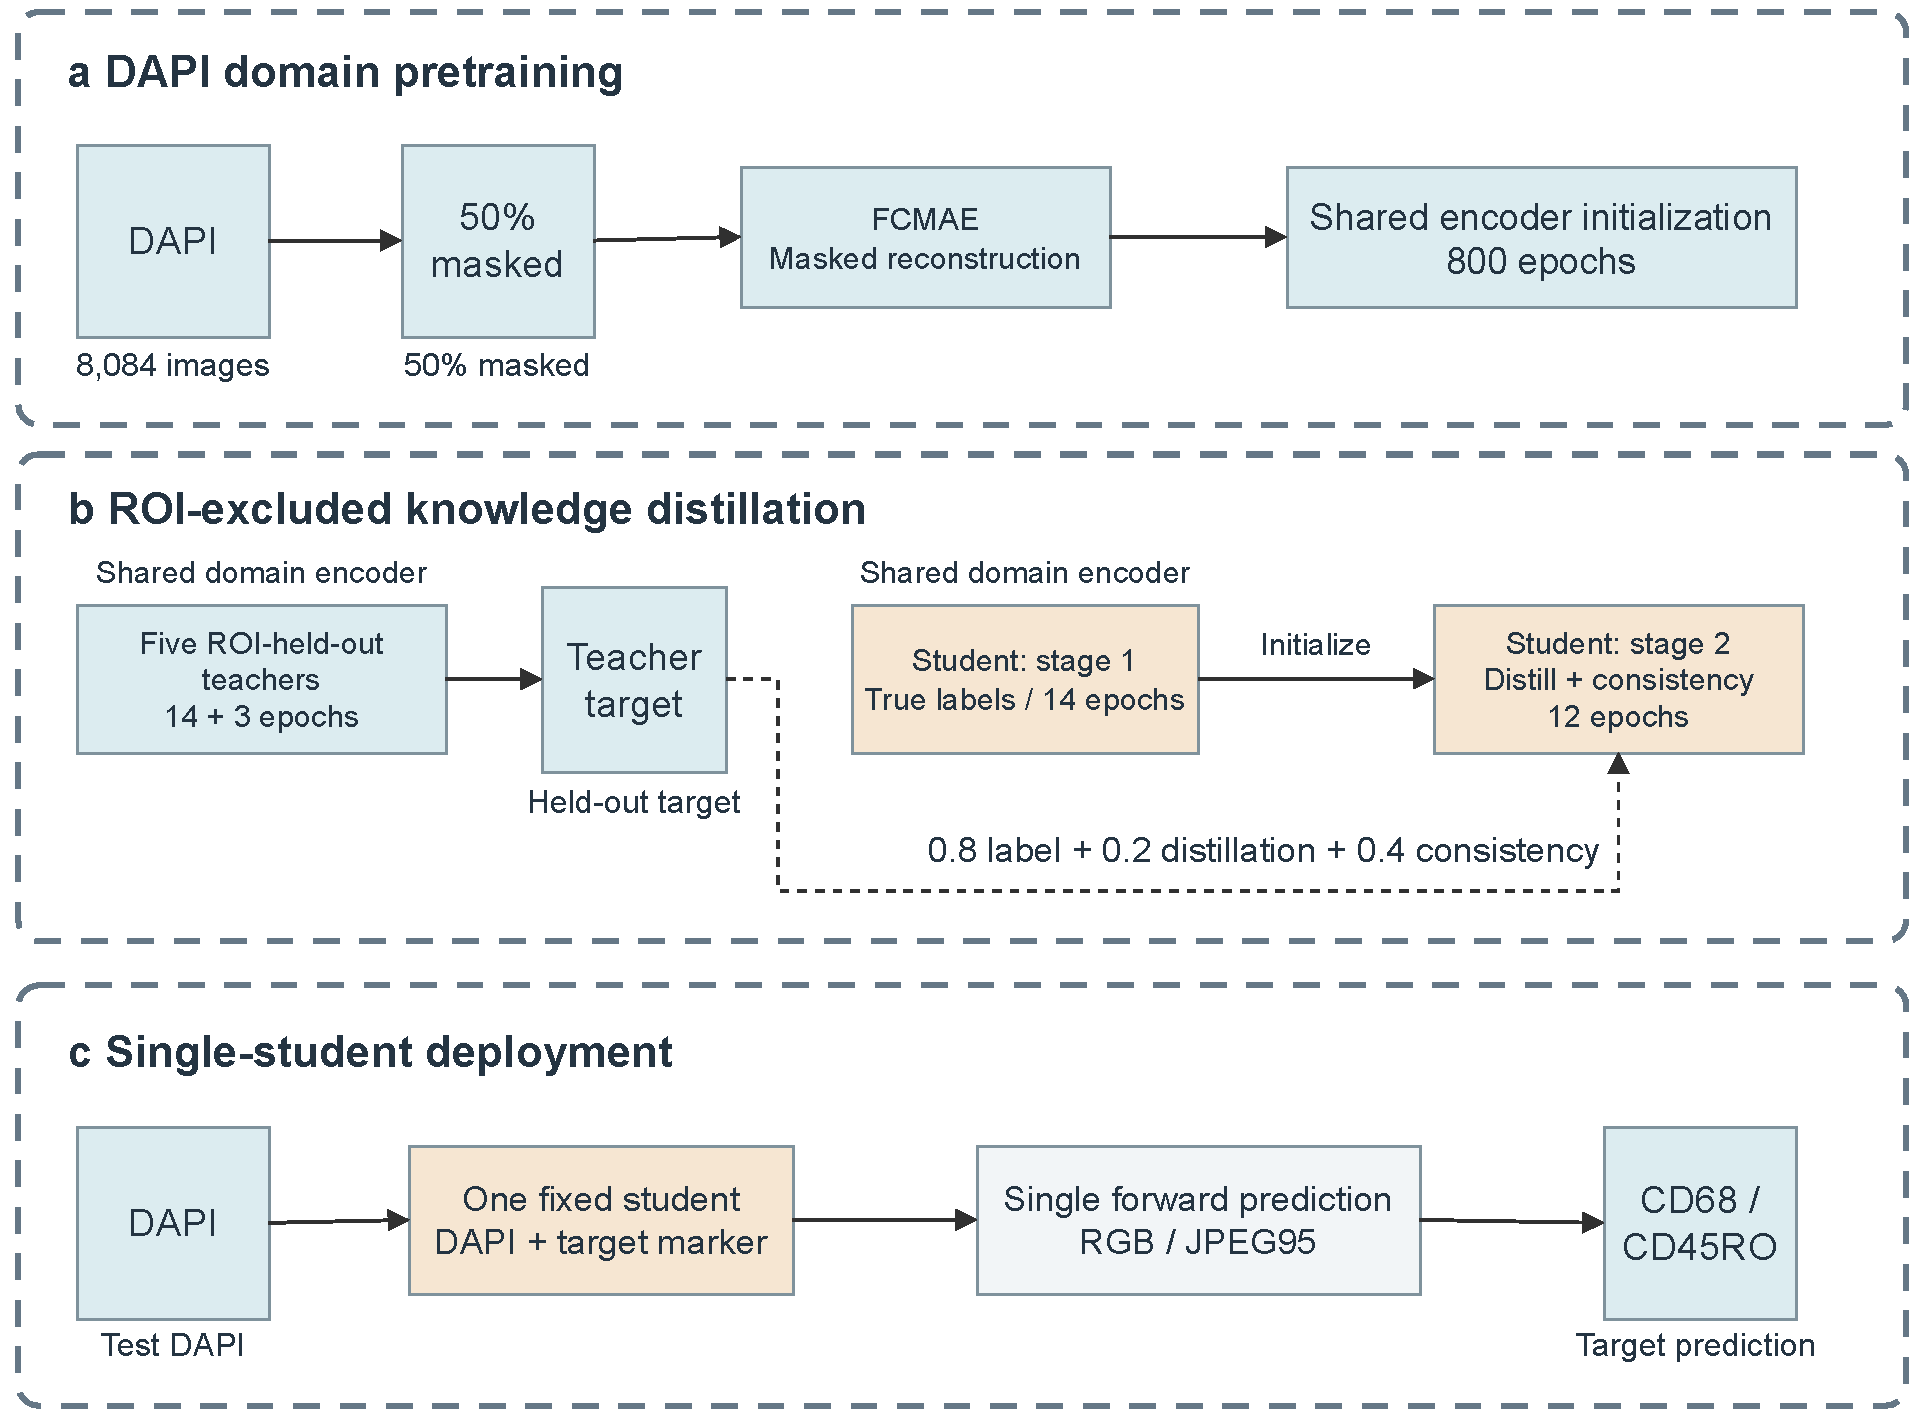
\includegraphics[width=\linewidth]{figures/workflow.pdf}
\caption{域内预训练、教师目标生成与全量学生学习流程。教师和学生共享域内编码器初始化；教师目标按 ROI 排除监督标签生成，每张图像对应一个教师。学生的任务层从固定随机种子初始化。}\label{fig:workflow}
\end{figure}

本文按“数据约定—单次前向结构—参数学习—部署推理—实验分析”的顺序展开。第\ref{sec:data}节说明 ROI 划分；第\ref{sec:model}节沿输入到输出介绍网络；第\ref{sec:training}节说明预训练、教师目标与学生优化；第\ref{sec:inference}节给出固定模型的推理过程；第\ref{sec:results}节分析验证与平台结果；第\ref{sec:discussion}节总结方法特点和局限。

\section{数据与组织区域划分}\label{sec:data}
本节确定后续网络输入和训练验证所依据的数据范围。三个器官均使用半决赛官方训练集和测试输入，每张 DAPI 与目标标记图像按名称一一对应。图块尺寸为 $256\times256$，ROI 标识用于划分训练与验证区域。各器官的数据规模见表\ref{tab:split}。

\begin{table}[H]\centering\small
\caption{官方数据与固定外层划分。训练、验证图块均来自官方训练集。}\label{tab:split}
\begin{tabular}{lrrrrl}\toprule
器官 & 训练集 ROI & 外层训练图块 & 验证图块 & 测试图块 & 目标标记\\\midrule
结肠 &25&5,004&1,292&1,346&CD68\\
肝脏 &17&1,820&560&560&CD45RO\\
胃 &12&1,260&420&280&CD68\\\midrule
合计 &54&8,084&2,272&2,186&\\\bottomrule
\end{tabular}
\end{table}

各器官内按完整 ROI 分组，以种子 2026 打乱 ROI 顺序，取前 20\%（向上取整）作为外层验证区域，其余用于参数学习。域内预训练使用这 8,084 张训练 DAPI；监督方案在同一组 2,272 张验证图像上比较。全量学生训练阶段合并官方训练集中的两部分，共使用 10,356 张配对图像。

教师的监督划分在外层训练 ROI 内进一步进行。首先按图块数对 ROI 排序，再将完整 ROI 分配给当前图块数最少的组，形成五组。每个教师排除其中一组的监督标签，为该组图像生成回归目标。外层验证 ROI 的标签同样由五个教师共同排除；全量学生训练时，将这些 ROI 按固定顺序逐组分配给一个教师生成目标。教师之间共享由外层训练 DAPI 学得的域内编码器，因此这一划分描述的是监督标签的排除关系。

\FloatBarrier
\section{从 DAPI 输入到标记图像输出}\label{sec:model}
在上述数据约定下，本节说明网络的一次前向计算。主路径依次为单张输入、四级编码、标记条件调制、逐级解码和单通道输出。条件路径将目标标记编号映射为各尺度的缩放与偏置，与编码特征汇合后进入解码器。
\subsection{输入与张量约定}
将完整单张 DAPI 转换为单通道灰度，并进行固定数值归一化：
\begin{equation}
x=I/255,\qquad \hat y=f_\theta(x,m).
\label{eq:input}
\end{equation}
\sym{其中，$I\in\{0,\ldots,255\}^{1\times256\times256}$ 为 DAPI 灰度图像，$x\in[0,1]^{1\times256\times256}$ 为网络输入；$m$ 为目标标记编号，CD68 和 CD45RO 分别对应 0 和 1；$f_\theta$ 为参数为 $\theta$ 的共享网络，$\hat y\in[0,1]^{1\times256\times256}$ 为目标标记预测。}
下文省略批量维，特征尺寸按“通道数 $\times$ 高 $\times$ 宽”书写；所有卷积和线性映射的参数均在训练中学习。图\ref{fig:architecture}展示完整前向结构。

\begin{figure}[htbp]\centering
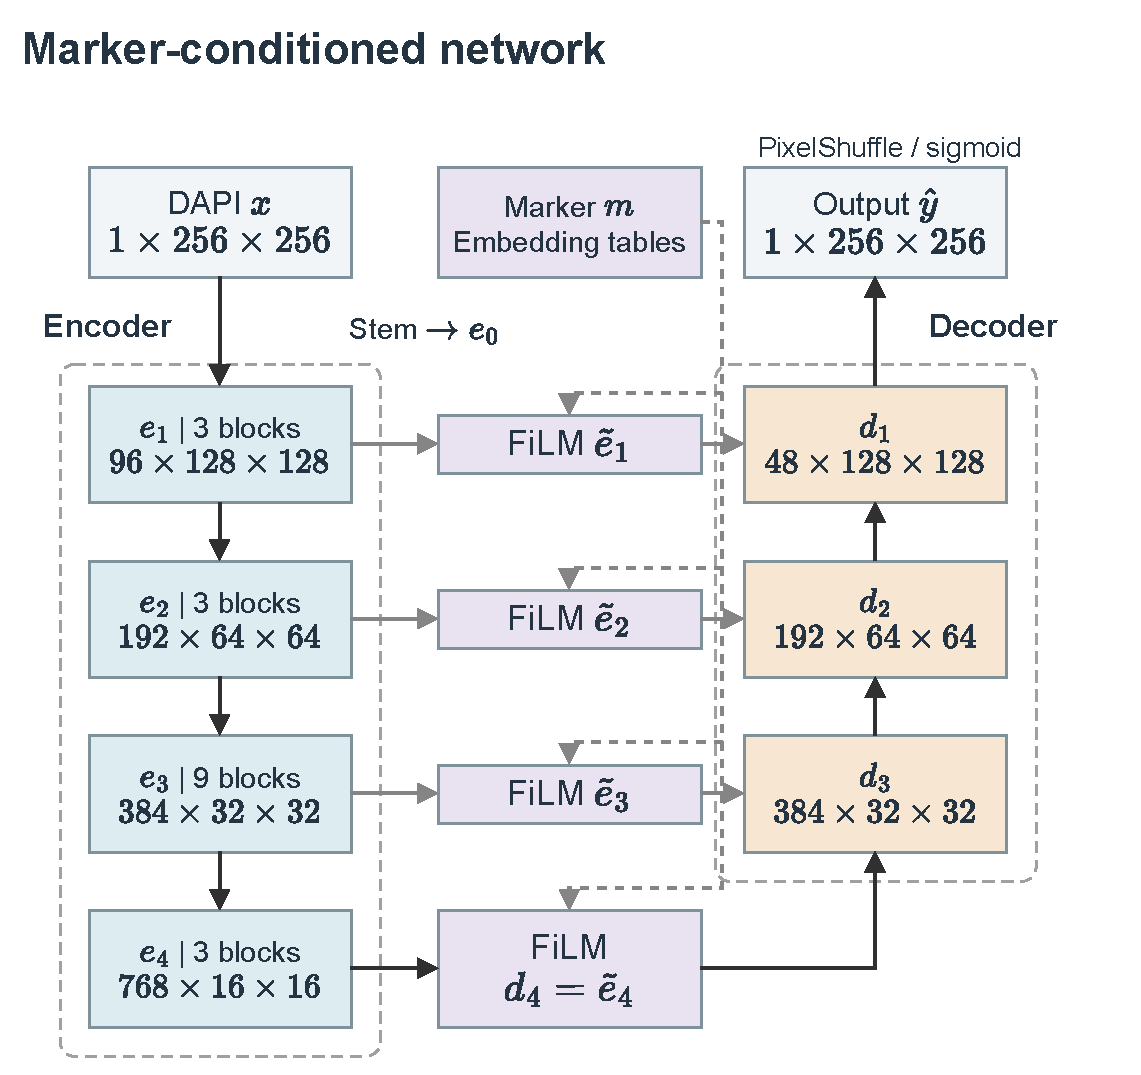
\includegraphics[width=\linewidth]{figures/architecture.pdf}
\caption{标记条件虚拟染色网络。四级编码特征分别进行 FiLM 调制，最深特征作为解码起点，其余特征通过同尺度跳跃连接参与融合。每级解码包含像素重排、拼接、归一化、通道投影和两个残差块；虚线表示标记条件。}\label{fig:architecture}
\end{figure}
\subsection{输入投影与四级编码器}
由上一小节得到的归一化输入 $x$ 首先进入输入投影层。该层由 $2\times2$、步长 2 的卷积和 LayerNorm 组成，将单通道图像映射为 96 通道特征。四级编码器继续构建分辨率递减的特征：
\begin{equation}
\begin{aligned}
e_0&=\op{LN}\bigl(\op{Conv}_{2,2}^{1\to96}(x)\bigr),\\
e_j&=\mathcal B_j^{[n_j]}\bigl(\mathcal A_j(e_{j-1})\bigr),
\quad j=1,2,3,4.
\end{aligned}
\label{eq:encoder}
\end{equation}
\sym{其中，$e_0$ 为输入投影特征，$e_j$ 为第 $j$ 个编码阶段的输出；$\op{Conv}_{k,s}^{a\to b}$ 表示核大小 $k$、步长 $s$、输入输出通道为 $a,b$ 的卷积；$\op{LN}$ 表示逐空间位置的通道 LayerNorm。$\mathcal A_1$ 为恒等映射，$\mathcal A_j$（$j\ge2$）依次执行 LN 和 $2\times2$ 步长 2 卷积；$\mathcal B_j^{[n_j]}$ 表示顺序堆叠 $n_j$ 个该阶段的 ConvNeXt V2 块。}
四阶段块数为 $(3,3,9,3)$，通道数为 $(96,192,384,768)$。对边长 $L=256$ 的输入，各阶段边长依次为 $L/2,L/4,L/8,L/16$；浅层特征同时保留给解码器跳跃连接。

\subsection{ConvNeXt V2 块内计算}
上述编码阶段中的 $\mathcal B_j$ 均由 ConvNeXt V2 块组成，解码器也复用这一基本单元，结构见图\ref{fig:blocks}。每个块先做 $7\times7$ 深度卷积，再进行通道归一化与四倍扩展，最后通过 GRN 和线性投影完成残差更新：
\begin{equation}
\begin{aligned}
v&=\op{DWConv}_{7,1}(u),\\
a&=\phi\bigl(W_1\op{LN}(v)+b_1\bigr),\\
\mathcal B(u)&=u+W_2\op{GRN}(a)+b_2.
\end{aligned}
\label{eq:block}
\end{equation}
\sym{其中，$u\in\mathbb R^{C\times H\times W}$ 为块输入，$C,H,W$ 为其通道数和空间尺寸；$v$ 为逐通道深度卷积输出；$W_1,b_1$ 将每个位置的通道从 $C$ 扩展至 $4C$，$W_2,b_2$ 将其投影回 $C$。$a$ 为扩展后的激活特征；$\phi(t)=t\Phi(t)$ 为 GELU，$\Phi$ 为标准正态累积分布函数；$\op{GRN}$ 为全局响应归一化，$\mathcal B(u)$ 为块输出。}

LayerNorm\cite{layernorm}作用于每个空间位置的通道向量：
\begin{equation}
\op{LN}(v)_{c,p}=\lambda_c
\frac{v_{c,p}-\mu_p}{\sqrt{\nu_p+\epsilon_{\rm LN}}}+\delta_c.
\label{eq:ln}
\end{equation}
\sym{其中，$c$ 为通道索引，$p$ 为空间位置；$v_{c,p}$ 为该位置的特征值，$\mu_p,\nu_p$ 为该位置所有通道的均值和总体方差；$\lambda_c,\delta_c$ 为可学习仿射参数，$\epsilon_{\rm LN}=10^{-6}$ 为数值稳定常数。}

GRN 对每个扩展通道汇总空间响应，并用通道平均响应归一化\cite{convnext}：
\begin{equation}
\begin{aligned}
g_c&=\sqrt{\sum_p a_{c,p}^2},\qquad
r_c=\frac{g_c}{\frac{1}{C_a}\sum_{k=1}^{C_a}g_k+\epsilon_g},\\
\op{GRN}(a)_{c,p}&=a_{c,p}+\alpha_c a_{c,p}r_c+\beta_c.
\end{aligned}
\label{eq:grn}
\end{equation}
\sym{其中，$a_{c,p}$ 为式\eqref{eq:block}的扩展特征，$C_a=4C$ 为扩展通道数；$g_c$ 为第 $c$ 通道的空间二范数，$k$ 为求平均时的通道索引，$r_c$ 为归一化响应；$\alpha_c,\beta_c$ 为零初始化的可学习参数，$\epsilon_g=10^{-6}$。}
深度卷积保留空间局部运算，通道扩展与投影完成特征混合，残差路径维持输入信息。编码器和解码器共使用 24 个此类块。


\begin{figure}[htbp]\centering
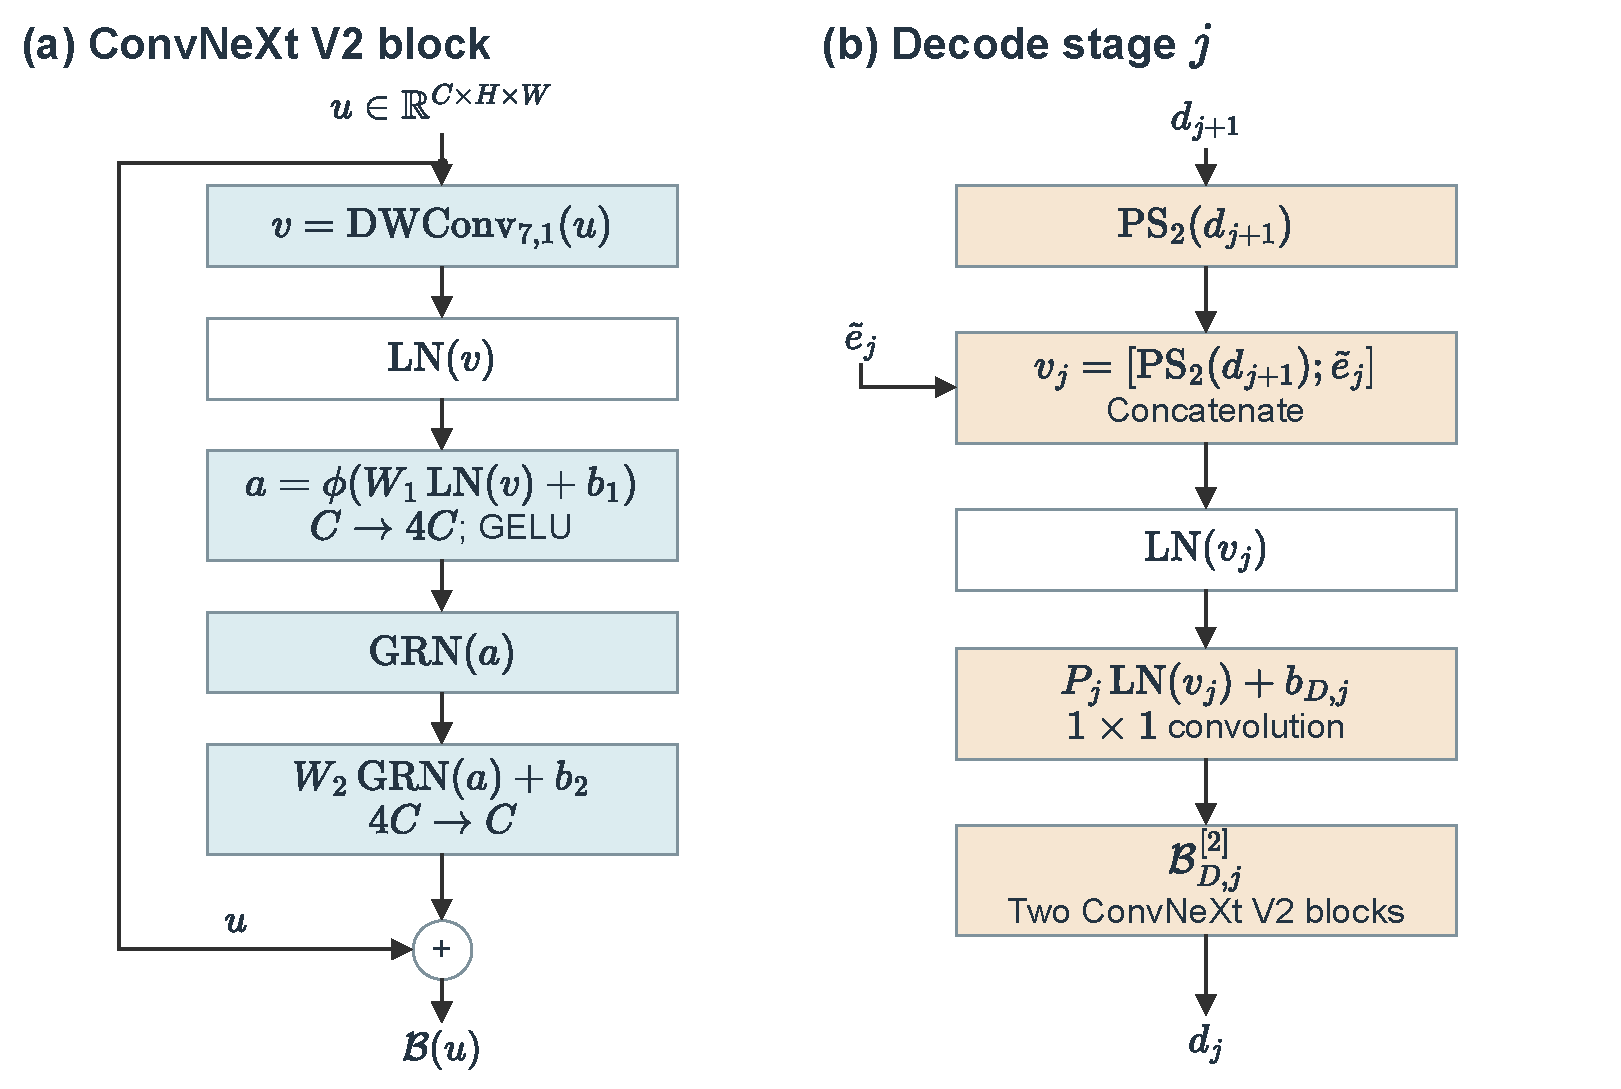
\includegraphics[width=.95\linewidth]{figures/blocks.pdf}
\caption{ConvNeXt V2 基本块与解码阶段。左侧为残差块内计算，右侧为结合标记调制特征的上采样与融合。}\label{fig:blocks}
\end{figure}

\subsection{标记嵌入与多尺度调制}
四级编码特征分别接受目标标记条件。对每个编码尺度设置一个独立嵌入表，将目标编号映射为逐通道仿射参数：
\begin{equation}
[\gamma_j(m);\beta_j(m)]=E_j[m],\qquad
\widetilde e_{j,c,p}=(1+\gamma_{j,c}(m))e_{j,c,p}+\beta_{j,c}(m).
\label{eq:film}
\end{equation}
\sym{其中，$j=1,\ldots,4$ 为编码尺度，$E_j\in\mathbb R^{4\times2C_j}$ 为该尺度的可学习嵌入表，$[\,;\,]$ 表示拼接；$\gamma_j(m),\beta_j(m)\in\mathbb R^{C_j}$ 分别为目标标记 $m$ 的缩放增量和偏置，$C_j\in\{96,192,384,768\}$；$c,p$ 为通道和空间位置，$\widetilde e_j$ 为调制后的特征。}
嵌入参数以标准差 0.01 的正态分布初始化，调制参数在同一特征图的空间位置间共享。各器官使用同一组编码器、嵌入表和解码器；结肠与胃的 CD68 任务使用相同的标记编号。

\subsection{跳跃连接与像素重排解码}
条件信息注入后，$\widetilde e_4$ 成为解码器的起点。解码器逐级恢复空间分辨率，并与同样经过调制的 $\widetilde e_3,\widetilde e_2,\widetilde e_1$ 融合：
\begin{equation}
\begin{aligned}
d_4&=\widetilde e_4,\quad
v_j=[\op{PS}_2(d_{j+1});\widetilde e_j],\\
d_j&=\mathcal B_{D,j}^{[2]}\bigl(P_j\op{LN}(v_j)+b_{D,j}\bigr),
\quad j=3,2,1.
\end{aligned}
\label{eq:decoder}
\end{equation}
\sym{其中，$d_j$ 为第 $j$ 尺度的解码特征，$\op{PS}_2$ 为二倍 PixelShuffle，$\widetilde e_j$ 为同尺度调制特征，$v_j$ 为通道拼接结果；$P_j,b_{D,j}$ 为 $1\times1$ 卷积权重及偏置，$\mathcal B_{D,j}^{[2]}$ 为两个串联的 ConvNeXt V2 块。}
三级拼接通道依次为 $192+384=576$、$96+192=288$ 和 $48+96=144$，经投影后依次得到 384、192、48 通道。每级先上采样，再利用浅层特征补充相应空间尺度的信息。

PixelShuffle 将通道位置重排为空间位置\cite{espcn}，二倍重排的索引定义为
\begin{equation}
\op{PS}_2(A)_{c,2i+a,2j+b}=A_{4c+2a+b,i,j}.
\label{eq:ps}
\end{equation}
\sym{其中，$A\in\mathbb R^{4C\times H\times W}$ 为输入张量，输出尺寸为 $C\times2H\times2W$；$c=0,\ldots,C-1$ 为输出通道，$i,j$ 为原空间坐标，$a,b\in\{0,1\}$ 为子像素偏移。该重排算子的可学习参数量为零。}
各解码阶段最后一个块的通道投影采用 ICNR 思路\cite{icnr}初始化：每组四个连续输出通道共享同一随机权重行，偏置置零，对应后续二倍重排的四个子像素位置。其余新建主干卷积和线性层使用标准差 0.02 的截断正态初始化。


\subsection{单通道输出与模块规模}
三级解码结束时，$d_1$ 为 48 通道、$128\times128$ 的特征图。输出层先做二倍像素重排，再通过两层卷积完成灰度映射：
\begin{equation}
\hat y=\sigma\!\left(K_2*\phi(K_1*\op{PS}_2(d_1)+b_1^{\mathrm{out}})+b_2^{\mathrm{out}}+b(m)\right).
\label{eq:output}
\end{equation}
\sym{其中，$\op{PS}_2(d_1)\in\mathbb R^{12\times256\times256}$ 为重排结果；$K_1$ 为 $3\times3$ 卷积，将 12 通道映射为 32 通道，采用一像素填充；$K_2$ 为 $1\times1$ 卷积，将 32 通道映射为 1 通道，$b_1^{\mathrm{out}},b_2^{\mathrm{out}}$ 为对应卷积偏置；$*$ 为卷积运算；$\phi$ 为 GELU，$b(m)$ 为初始值 $-2$ 的标记相关标量偏置，$\sigma(t)=1/(1+e^{-t})$ 为 Sigmoid。}
卷积输出头采用 PyTorch 的默认初始化，输出空间尺寸与输入一致。上述路径的逐模块参数量见表\ref{tab:params}；网络总参数量为 31,228,917，约 31.23M。

\begin{table}[H]\centering\small
\caption{最终学生网络的模块参数量和输出尺寸。编码阶段包含入口下采样，解码阶段包含融合投影及两个残差块。}\label{tab:params}
\begin{tabularx}{\textwidth}{lYrr}\toprule
模块 & 主要配置 & 输出尺寸 & 参数量\\\midrule
输入投影 & $2\times2$ 步长 2 卷积；LN & $96\times128\times128$ &672\\
编码阶段 1 &3 个 ConvNeXt V2 块&$96\times128\times128$&239,904\\
编码阶段 2 &下采样；3 个块&$192\times64\times64$&996,288\\
编码阶段 3 &下采样；9 个块&$384\times32\times32$&11,137,152\\
编码阶段 4 &下采样；3 个块&$768\times16\times16$&15,486,720\\
标记嵌入 &四尺度 FiLM 参数表&对应各编码尺度&11,520\\\midrule
解码阶段 3 &拼接后投影 $576\to384$&$384\times32\times32$&2,631,936\\
解码阶段 2 &拼接后投影 $288\to192$&$192\times64\times64$&670,848\\
解码阶段 1 &拼接后投影 $144\to48$&$48\times128\times128$&50,352\\
输出头 &重排；卷积 $12\to32\to1$&$1\times256\times256$&3,521\\
标记输出偏置 &标量嵌入表&1&4\\\midrule
\textbf{总计} &\multicolumn{2}{l}{共享条件网络}&\textbf{31,228,917}\\\bottomrule
\end{tabularx}
\end{table}

\FloatBarrier
\section{域内预训练与知识蒸馏}\label{sec:training}
第\ref{sec:model}节定义了网络如何生成标记图像，本节说明这些映射参数如何学习。训练包含域内预训练、教师监督学习与目标生成、全量学生学习三个环节。教师和学生共享固定的域内编码器初始化，任务层以种子 2026 初始化。下文依次给出预训练目标、监督损失、教师到学生的目标传递，以及各环节的优化设置。
\subsection{公开初始化及域内预训练}
训练从 ConvNeXt V2 Tiny 的 ImageNet-1K FCMAE 公开权重开始\cite{convnext}。本模型的单通道 $2\times2$ 输入卷积按固定种子初始化，其余形状兼容的编码器参数从公开权重加载。随后在固定外层训练划分的 8,084 张 DAPI 上进行 800 轮域内预训练，所得编码器用于全部教师和最终学生。

掩码在编码器最深尺度的 $16\times16$ 网格上生成（每个网格位置对应输入的 $16\times16$ 像素区域），每张输入随机遮蔽 50\% 的网格位置，并按整数倍扩展至各特征尺度。实现采用密集张量与可见位置掩码：输入层、下采样层和块内卷积前后按可见掩码限制特征传播。预训练解码器沿用三级像素重排结构，每级使用一个块，输出一个 DAPI 重建通道。掩码区域损失为
\begin{equation}
\mathcal L_{\rm pre}=\frac{\sum_p M_p(\widetilde x_p-x_p)^2}
{\sum_p M_p}.
\label{eq:pretrain}
\end{equation}
\sym{其中，$x$ 为预训练使用的归一化 $256\times256$ DAPI 图块，$\widetilde x$ 为重建输出，$p$ 为像素位置；$M_p\in\{0,1\}$ 表示该位置属于遮蔽区域时为 1，$\mathcal L_{\rm pre}$ 为遮蔽像素上的平均平方误差。预训练完成后将编码器参数用于监督网络初始化。}
公开权重提供初始表征，域内重建训练使编码器适应本次 DAPI 的强度和形态分布。训练 DAPI 的旋转、翻转增强与掩码采样共同产生预训练样本。

\subsection{结构与像素强度联合损失}
完成域内预训练后，网络转入 DAPI 到免疫标记图像的监督学习。教师和学生共用以下结构与像素强度损失。结构相似性指标 SSIM\cite{ssim}约束局部图像结构，其窗口形式为
\begin{equation}
\op{SSIM}(a,b)=
\frac{(2\mu_a\mu_b+C_1)(2\sigma_{ab}+C_2)}
{(\mu_a^2+\mu_b^2+C_1)(\sigma_a^2+\sigma_b^2+C_2)}.
\label{eq:ssim}
\end{equation}
\sym{其中，$a,b$ 为同位置的预测和标签窗口，$\mu_a,\mu_b$ 为窗口均值，$\sigma_a^2,\sigma_b^2$ 为窗口方差，$\sigma_{ab}$ 为协方差；对 $[0,1]$ 图像取 $C_1=0.01^2,C_2=0.03^2$。图像 SSIM 为有效窗口位置的局部值均值。训练使用 $7\times7$ 均匀窗口及 $49/48$ 的样本协方差修正。}

单通道混合损失为
\begin{equation}
\begin{aligned}
\ell(\hat y,y)={}&0.7\bigl(1-\op{SSIM}_7(\hat y,y)\bigr)\\
&+\frac{0.2}{P}\sum_p|\hat y_p-y_p|
+\frac{0.1}{P}\sum_p(\hat y_p-y_p)^2.
\end{aligned}
\label{eq:loss}
\end{equation}
\sym{其中，$\hat y,y$ 为同尺寸的单通道预测与标签，$P$ 为该通道参与像素损失的像素总数，$p$ 为像素索引；$\op{SSIM}_7$ 为前述均匀 7 窗口图像 SSIM。三项分别约束局部结构、平均绝对误差和平均平方误差。}


三个器官的样本共同参与监督学习，逐图损失按官方综合评价中的器官权重加权：
\begin{equation}
w_o=(0.1,0.2,0.7)_o,\qquad a_o=\frac{Nw_o}{N_o},\qquad
\mathcal L_{\rm label}=\frac1N\sum_{i=1}^{N}a_{o(i)}\ell(\hat y_i,y_i).
\label{eq:organloss}
\end{equation}
\sym{其中，$o$ 按结肠、肝脏、胃排列，$w_o$ 为器官权重；$N$ 为当前训练范围的图像总数，$N_o$ 为器官 $o$ 的图像数，$a_o$ 为其逐图损失系数；$i$ 为样本索引，$o(i)$ 为样本所属器官，$\hat y_i,y_i$ 为所选标记的预测和标签。}
每轮将当前训练范围的图像打乱后逐一遍历，损失系数使三个器官的平均贡献与给定权重对应。器官信息在训练中用于确定损失权重，目标标记编号用于网络条件调制。

\subsection{教师目标生成与学生学习}
本方案采用输出层知识蒸馏\cite{distill}，以教师预测的连续灰度图像作为辅助回归目标。五个教师使用同一结构与训练参数，各自进行第一阶段 14 轮和第二阶段 3 轮监督训练，统一采用第 17 轮参数。教师预测保留为 8 位灰度目标：
\begin{equation}
t_i=\frac1{255}\op{round}\!\left(255 f_{\theta^{T}_{k(i)}}(x_i,m_i)\right).
\label{eq:target}
\end{equation}
\sym{其中，$x_i,m_i$ 为样本 $i$ 的归一化 DAPI 与目标标记编号；$k(i)$ 为按第\ref{sec:data}节划分指定的教师，$\theta^{T}_{k(i)}$ 为该教师的固定参数，其监督训练排除了样本所属 ROI 的标签；$\op{round}$ 为最近整数舍入（半整数取相邻偶数），$t_i$ 为量化后恢复到 $[0,1]$ 的教师目标。}
汇集教师预测后，全部 10,356 张官方训练图像各有一个目标。全量学生使用这些配对图像，先以真实标签完成第一阶段训练，再在第二阶段加入固定教师目标。

与此同时，第二阶段引入几何一致性约束。对一次训练样本执行额外的旋转或翻转，将预测恢复到原坐标后与原视角预测比较：
\begin{equation}
\mathcal L_{{\rm geo},i}=\ell\!\left(f_\theta(x_i,m_i),
g_i^{-1}f_\theta(g_ix_i,m_i)\right).
\label{eq:consistency}
\end{equation}
\sym{其中，$g_i$ 为八元素 D4 集合中的一个非恒等变换，由训练轮次和样本次序按固定规则确定；D4 包含四种 $90^\circ$ 整数倍旋转及其镜像，$g_i^{-1}$ 为对应逆变换；$\ell$ 为式\eqref{eq:loss}的图像损失，两次前向计算共享学生参数并共同参与反向传播。}
该项约束染色映射随空间变换保持协调，辅助学生学习稳定的结构响应。第二阶段的完整目标为
\begin{equation}
\mathcal L_{\rm stu}=\frac1N\sum_{i=1}^{N}a_{o(i)}
\left[0.8\ell(\hat y_i,y_i)+0.2\ell(\hat y_i,t_i)+0.4\mathcal L_{{\rm geo},i}\right].
\label{eq:student}
\end{equation}
\sym{其中，$N,a_{o(i)}$ 沿用式\eqref{eq:organloss}，$\hat y_i=f_\theta(x_i,m_i)$ 为当前学生预测，$y_i$ 为真实标签，$t_i$ 为固定教师目标，$\mathcal L_{{\rm geo},i}$ 为式\eqref{eq:consistency}。训练中输入、真实标签和教师目标先接受相同的随机几何增强，再计算上述损失。}

\subsection{优化设置与阶段衔接}
上述各环节使用 AdamW\cite{adamw} 优化，根随机种子固定为 2026，具体设置见表\ref{tab:training}。教师与学生均采用两阶段监督训练，第二阶段从各自第一阶段第 14 轮参数及随机状态开始，重新创建优化器与学习率周期。全量学生采用验证选定的第 26 轮，即第二阶段第 12 轮参数。

监督阶段按余弦规律衰减学习率\cite{sgdr}，并按编码器深度设置倍率，使浅层参数以较小步长更新：
\begin{equation}
\eta_j(e)=\rho_j\frac{\eta_0}{2}\left[1+\cos\!\left(\frac{\pi(e-1)}{14}\right)\right],
\qquad \rho_j=0.8^{4-j},\quad j=0,\ldots,4.
\label{eq:lr}
\end{equation}
\sym{其中，$e\in\{1,\ldots,14\}$ 为阶段内轮次，$\eta_0$ 为该阶段基础学习率；$j=0$ 对应输入投影，$j=1,\ldots,4$ 对应四级编码阶段；$\rho_j$ 为深度学习率倍率，解码器、输出头与标记嵌入使用倍率 1。}
教师与学生均采用上述分层设置。两个阶段的余弦周期固定为 14 轮；教师第二阶段在第 3 轮结束，最终学生第二阶段在第 12 轮结束。每轮随机打乱样本，监督增强对 DAPI、真实标签及教师图像同步执行旋转和翻转。每个优化器更新累积 16 张图像的梯度，梯度范数裁剪阈值为 1。

\begin{table}[H]\centering\small
\caption{训练参数。有效批量为微批量乘梯度累积次数。}\label{tab:training}
\begin{tabularx}{\linewidth}{lYY}\toprule
项目 & 域内预训练 & 监督训练\\\midrule
轮次 &800&教师 $14+3$；最终学生 $14+12$\\
微批量 / 累积 &1 / 32&1 / 16\\
基础学习率 &$2\times10^{-4}$&$3\times10^{-4}$；$10^{-4}$\\
权重衰减 &0.05&$10^{-4}$\\
调度 &10 轮预热，余弦至 $10^{-6}$&每阶段固定 14 轮余弦周期\\
输入边长 &256&256\\
目标 &遮蔽位置 MSE&结构与强度损失、蒸馏及一致性\\
掩码比例 &0.5&完整输入\\
精度 &BF16 前向，FP32 损失&BF16 前向，FP32 损失\\\bottomrule
\end{tabularx}
\end{table}

\FloatBarrier
\section{固定模型推理}\label{sec:inference}
上一节得到一个全量训练的学生模型。本节说明如何固定其参数，将第\ref{sec:model}节的前向计算用于测试图像。所有任务共用同一学生权重，模型置于评估模式，以 FP32 对完整单张 DAPI 和指定标记编号执行一次前向计算。结肠与胃任务指定 CD68，肝脏任务指定 CD45RO。

预测图像执行固定保存转换：
\begin{equation}
J_i=\op{RGB}\left(\op{uint8}\left[
\op{clip}\bigl(\op{round}(255\hat y_i),0,255\bigr)\right]\right).
\label{eq:save}
\end{equation}
\sym{其中，$\hat y_i$ 为第 $i$ 张 $256\times256$ 预测图像，$\op{round}$ 为最近整数舍入（半整数取相邻偶数），$\op{clip}$ 将数值限制在给定闭区间，$\op{uint8}$ 为 8 位无符号整数转换，$\op{RGB}$ 将灰度复制到三个颜色通道，$J_i$ 为待保存图像。JPEG 保存质量固定为 95。}
输出保持输入的视野、方向、尺寸和逐图对应关系，三个器官共生成 2,186 张目标图像。

\FloatBarrier
\section{实验结果与分析}\label{sec:results}
本节先在固定外层 ROI 划分上考察蒸馏与几何一致性，再报告全量学生的平台表现。验证实验使用同一组区域和相同指标，最终训练采用验证选定的配置与轮次。
\subsection{实验环境与指标}
最终训练与推理使用 NVIDIA RTX5090、Windows、Python3.13.5 和 PyTorch2.8.0+cu128。分组验证按器官、图像和 ROI 汇总，三个器官分别包含 5、4、3 个验证 ROI。

本地验证采用 $11\times11$ 高斯窗口、标准差 1.5、总体协方差和有效窗口计算 SSIM。PSNR 在归一化像素尺度上计算，单图综合分以及跨器官加权分为
\begin{equation}
\begin{aligned}
\op{PSNR}_i&=-10\log_{10}\max\!\left(\frac1P\sum_p(\hat y_{i,p}-y_{i,p})^2,10^{-12}\right),\\
s_i&=70\op{SSIM}_i+0.6\min(\op{PSNR}_i,50),\\
S&=0.1\bar s_{\rm colon}+0.2\bar s_{\rm liver}+0.7\bar s_{\rm stomach}.
\end{aligned}
\label{eq:score}
\end{equation}
\sym{其中，$P$ 为图像像素数，$p$ 为像素索引；$\op{PSNR}_i$ 为第 $i$ 张图像的 PSNR，单位为 dB；$\hat y_{i,p},y_{i,p}$ 为编码后预测和标签在 $[0,1]$ 尺度的像素值，$s_i$ 为单图分数；$\bar s_o$ 为器官 $o$ 全部评价图像的平均分，$S$ 为三器官加权分。每个器官在本方案中对应一个目标标记。}
验证预测经固定 JPEG95 编码后计算指标。SSIM 衡量局部结构关系，PSNR 衡量平均平方误差；两者在单图分数中的权重分别为 70\% 和 30\%，PSNR 以 50 dB 归一化并封顶。

\subsection{蒸馏与几何一致性对照}
表\ref{tab:validation}汇总相同外层划分下的验证结果。基础配置已经采用固定域内编码器和器官加权监督；蒸馏将综合分数由 76.1035 提高至 76.2247，三个器官的平均分均改善，12 个验证 ROI 中有 9 个改善。

\begin{table}[H]\centering\small
\caption{固定 ROI 验证结果。各行报告固定配置的最佳验证分，几何一致性权重逐项列出。}\label{tab:validation}
\begin{tabularx}{\linewidth}{Yrr}\toprule
训练配置 & 一致性权重 & 综合分数\\\midrule
器官加权监督 &0&76.1035\\
加入教师蒸馏 &0&76.2247\\
蒸馏与几何一致性 &0.1&76.2500\\
蒸馏与几何一致性 &0.2&76.2672\\
蒸馏与几何一致性 &0.4&\textbf{76.2807}\\\bottomrule
\end{tabularx}
\end{table}

一致性权重由 0.2 提高到 0.4 后，最佳轮次均为第 26 轮，加权分数提高 0.01345。结肠、肝脏和胃的验证增益分别为 0.00469、0.02114 和 0.01251。14 个相同训练轮次中有 11 个分数更高，最后 9 轮连续高于对照，说明这一小幅收益同时体现在训练后段的走势中。

最终配置的分器官指标见表\ref{tab:organval}。胃的三个验证 ROI 中，两个分别提高 0.01705 和 0.02445，另一个下降 0.00398，区域间仍存在差异。上述增益来自同一固定划分，反映本次配对比较中的平均变化。

\begin{table}[H]\centering\small
\caption{最终配置的固定 ROI 验证指标。PSNR 为逐图封顶后的均值。}\label{tab:organval}
\begin{tabular}{llrrr}\toprule
器官&标记&SSIM&PSNR（dB）&综合分数\\\midrule
结肠&CD68&0.835873&26.553097&74.442950\\
肝脏&CD45RO&0.873513&27.400676&77.586285\\
胃&CD68&0.837292&29.266285&76.170192\\\bottomrule
\end{tabular}
\end{table}

\subsection{全量学生的平台结果}
按验证确定的第 26 轮和一致性权重 0.4，使用全部官方训练图像重新完成监督训练。最终平台结果见表\ref{tab:online}，三器官加权分数为 74.0677。

\begin{table}[H]\centering\small
\caption{最终全量学生的平台结果。}\label{tab:online}
\begin{tabular}{llrr}\toprule
器官&目标标记&评价权重&平台分数\\\midrule
结肠&CD68&0.1&73.1963\\
肝脏&CD45RO&0.2&78.7011\\
胃&CD68&0.7&72.8684\\\midrule
\multicolumn{3}{l}{\textbf{加权分数}}&\textbf{74.0677}\\\bottomrule
\end{tabular}
\end{table}

与一致性权重 0.2 的全量学生平台分数 74.0243 相比，最终配置提高 0.0434。结肠和胃分别提高 0.1711 和 0.0413，肝脏下降 0.0132。按评价权重计算，三者对综合变化的贡献约为 $+0.01711$、$-0.00264$ 和 $+0.02891$，主要增益来自结肠和胃。这里比较的是两套全量训练方案的最终结果，验证与平台评价的图像集合各自独立。

\FloatBarrier
\section{方法特点与局限}\label{sec:discussion}
结合前述结构、训练流程和实验结果，本节归纳方法的主要特点，并界定当前结果的适用范围。
\subsection{方法特点}
本方法将多尺度形态学习与目标标记条件结合在同一个预测网络中。共享编码器与解码器承担三个器官的图像映射，四尺度 FiLM 嵌入在每次前向中指定目标标记。跳跃连接补充浅层细节，像素重排逐级恢复分辨率，最终通过卷积输出头生成单通道染色图像。

参数学习与上述结构相配合。DAPI 域内掩码重建提供编码器初始化，器官加权监督将更新方向与三器官评价权重对应，ROI 留出教师目标为学生增加回归约束。几何一致性将方向变换前后的输出关系纳入训练目标，最终部署保留一条固定前向路径。该组合在固定验证划分上获得了持续的小幅改善，并形成约 31.23M 参数的共享学生模型。

\subsection{局限性}
当前数据包含 54 个训练 ROI，其中胃的验证集仅有 3 个 ROI，区域数量限制了微小收益的稳定性判断。验证集与测试集的器官分数差异也表明，组织区域分布会影响最终表现。DAPI 主要反映细胞核形态，目标免疫标记还涉及更复杂的组织成分与生物学状态，单张图像中的形态信息对染色强度的解释能力有限。

教师预测误差与 8 位量化误差会共同影响辅助目标的细节；几何一致性在增强方向稳定性的同时增加训练计算量，其权重需要在结构恢复与约束强度之间取得平衡。共享网络还需协调不同器官和标记的梯度，后续研究可围绕更充分的区域验证与形态相关表征改进展开。

\begin{thebibliography}{99}\small
\setlength{\itemsep}{1pt}
\bibitem{unet} O. Ronneberger, P. Fischer, and T. Brox. U-Net: Convolutional Networks for Biomedical Image Segmentation. MICCAI, 2015. \href{https://arxiv.org/abs/1505.04597}{arXiv:1505.04597}.
\bibitem{cytoland} Z. Liu, E. Hirata-Miyasaki, S. Pradeep, et al. Robust virtual staining of landmark organelles with Cytoland. Nature Machine Intelligence, 7:901--915, 2025. \href{https://doi.org/10.1038/s42256-025-01046-2}{doi:10.1038/s42256-025-01046-2}.
\bibitem{convnext} S. Woo, S. Debnath, R. Hu, et al. ConvNeXt V2: Co-designing and Scaling ConvNets with Masked Autoencoders. CVPR, 2023. \href{https://arxiv.org/abs/2301.00808}{arXiv:2301.00808}.
\bibitem{espcn} W. Shi, J. Caballero, F. Husz\'ar, et al. Real-Time Single Image and Video Super-Resolution Using an Efficient Sub-Pixel Convolutional Neural Network. CVPR, 2016. \href{https://arxiv.org/abs/1609.05158}{arXiv:1609.05158}.
\bibitem{film} E. Perez, F. Strub, H. de Vries, V. Dumoulin, and A. Courville. FiLM: Visual Reasoning with a General Conditioning Layer. AAAI, 2018. \href{https://arxiv.org/abs/1709.07871}{arXiv:1709.07871}.
\bibitem{layernorm} J. L. Ba, J. R. Kiros, and G. E. Hinton. Layer Normalization. arXiv, 2016. \href{https://arxiv.org/abs/1607.06450}{arXiv:1607.06450}.
\bibitem{icnr} A. Aitken, C. Ledig, L. Theis, et al. Checkerboard artifact free sub-pixel convolution: A note on sub-pixel convolution, resize convolution and convolution resize. arXiv, 2017. \href{https://arxiv.org/abs/1707.02937}{arXiv:1707.02937}.
\bibitem{ssim} Z. Wang, A. C. Bovik, H. R. Sheikh, and E. P. Simoncelli. Image Quality Assessment: From Error Visibility to Structural Similarity. IEEE Transactions on Image Processing, 13(4):600--612, 2004. \href{https://doi.org/10.1109/TIP.2003.819861}{doi:10.1109/TIP.2003.819861}.
\bibitem{distill} G. Hinton, O. Vinyals, and J. Dean. Distilling the Knowledge in a Neural Network. arXiv, 2015. \href{https://arxiv.org/abs/1503.02531}{arXiv:1503.02531}.
\bibitem{adamw} I. Loshchilov and F. Hutter. Decoupled Weight Decay Regularization. ICLR, 2019. \href{https://arxiv.org/abs/1711.05101}{arXiv:1711.05101}.
\bibitem{sgdr} I. Loshchilov and F. Hutter. SGDR: Stochastic Gradient Descent with Warm Restarts. ICLR, 2017. \href{https://arxiv.org/abs/1608.03983}{arXiv:1608.03983}.
\end{thebibliography}
\end{document}
